\chapter{Theoretical Background}
\label{chap:background}

This chapter provides the theory essential to understand the major components of the thesis. Prior knowledge of Artificial Neural Networks \footnote{Artificial Neural Networks \url{https://en.wikipedia.org/wiki/Artificial_neural_network}} and fundamental concepts of Deep Learning \cite{theory_dl} is assumed.

\section{Preliminary Concepts}
\label{sec:Preliminary}

\subsection{Autoencoder}
Autoencoders are a variant of \acp{ann}, which are designed to learn an identity function that generates the input data sample back. The network has a bottleneck($z$), dividing the network into two parts, an encoder and a decoder as illustrated in Fig \ref{fig:ae_arch}. The first network learns to compress the high dimensional input data to a low dimensional intermediate representation, \textit{latent representation}, at the bottleneck. While the second network learns to reconstruct the data from the latent distribution. Thus learning to efficiently compress the data.

\begin{figure}[h]
    \centering
    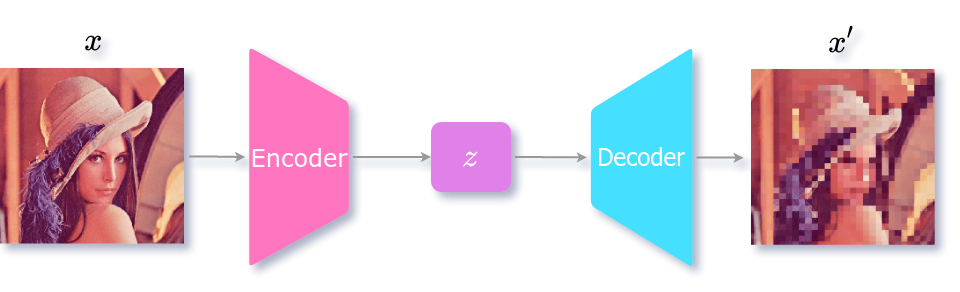
\includegraphics[width=0.8\textwidth]{figures/arch/ae_arch.png}
    \caption{Illustration of autoencoder architecture. Image source \cite{deepimageprior}}
    \label{fig:ae_arch}
\end{figure}

To put it in other words, in the process of learning to reconstruct the data, the encoder learns to filter the most important features of the given data distribution, so as it preserves the complete properties within the limits of the bottleneck. While the decoder learns comparatively general properties of the distribution which are used along with the compact latent representation from the encoder to fully recover the data distribution. The network is trained to minimize the similarity between the reconstruction and the original data sample. This similarity can be determined by metrics such as \ac{mse}, \ac{l1} or Cross-Entropy loss.

The idea of an autoencoder dates back to the '80s proposed as a method for pre-training and feature learning \cite{ballard1987modular, rumelhart1985learning}, learned dimensionality reduction \cite{hinton_dimentionality}. In recent years, autoencoders are most popularly used as generative networks leveraging their ability to learn feature representations in an unsupervised way. Another interesting variant of autoencoders is the denoising autoencoder \cite{vincent2008extracting}, where the input is a noised data and the decoder generates original data without noise. This variant is further evolved to accomplish the tasks of image denoising, watermark removal, inpainting, super-resolution, colorization, de-colorization, and compression \cite{zhang2016colorful, imagedenoisingpaper,deepimageprior}. 

\subsection{Variational Autoencoders}
\label{subsec:vae}
\acp{vae}, unlike standard autoencoders, learn to encode a data sample $x$ as a probabilistic distribution rather than a deterministic value for the latent attribute \footnote{\label{note:jeremy_jordan} Variational Autoencoders \url{https://www.jeremyjordan.me/variational-autoencoders/}}. The encoder $q$ produces the probabilistic distribution by predicting two vectors that represent the mean $\mu$ and standard deviation $\sigma$ of distribution for each of the latent attributes of $x$. And the decoder $p$ takes a random sample $z$ from this distribution to recover the sample as illustrated in Fig \ref{fig:vae_arch}.

\begin{figure}[h]
    \centering
    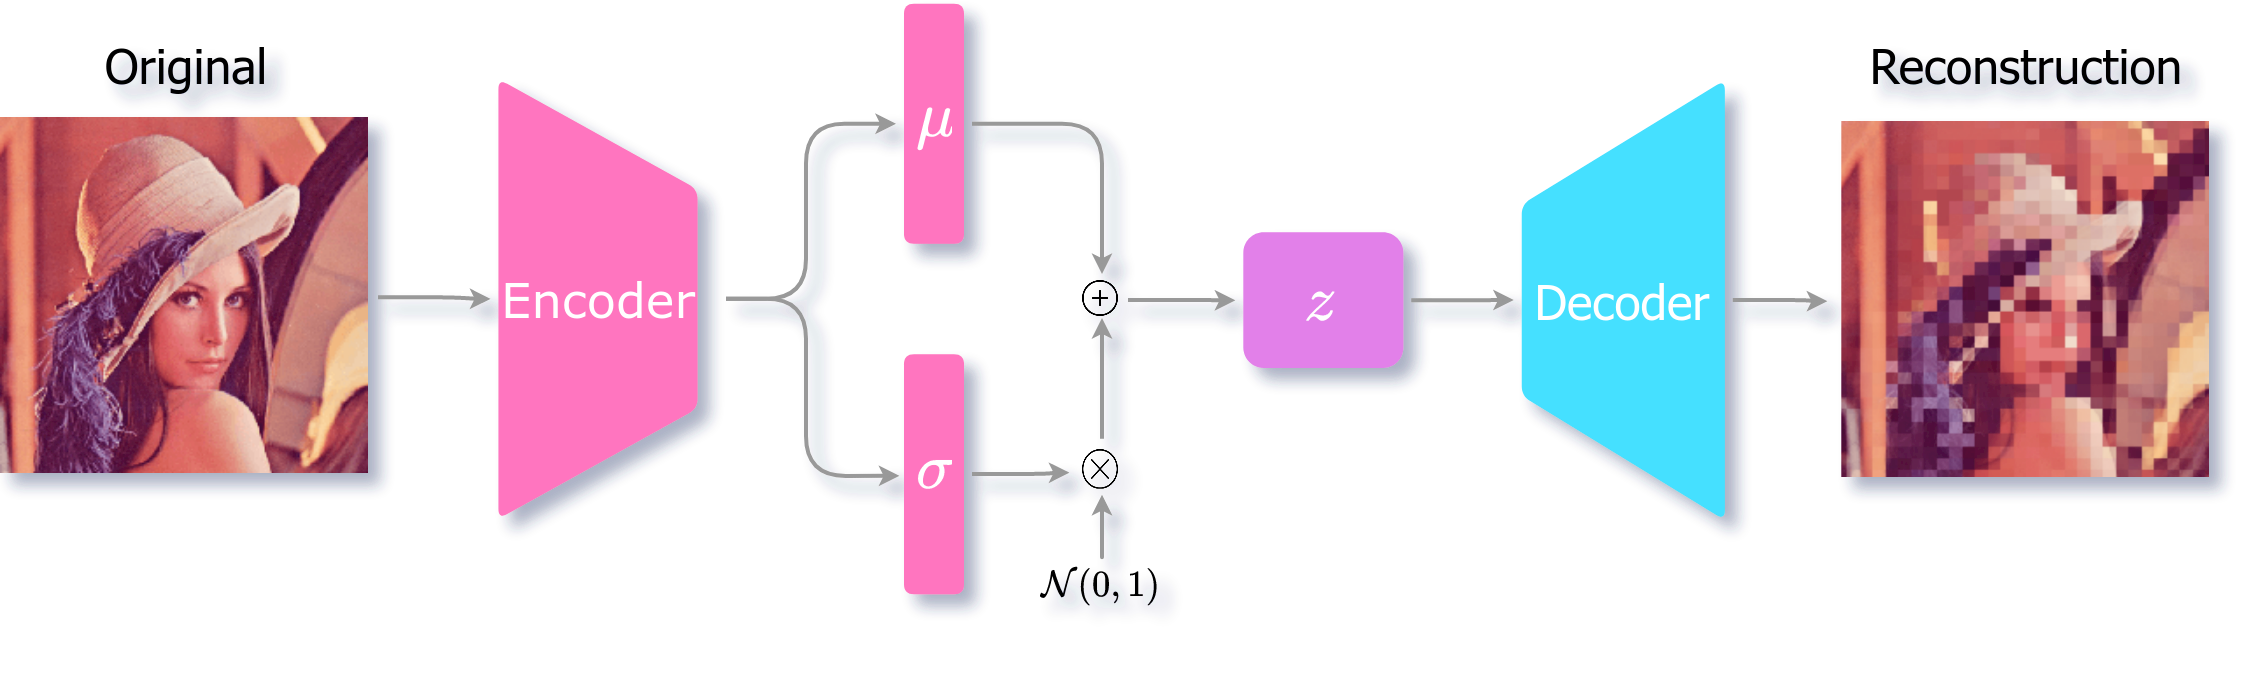
\includegraphics[width=\textwidth]{figures/arch/vae_arch.png}
    \caption{Illustration of Variational Autoencoder architecture.}
    \label{fig:vae_arch}
\end{figure}

To put it formally, we have a hidden variable $z$ which generates $x$. Since we only have $x$ and would want to learn $z$ i.e $p(z | x)$. But computing this posterior distribution is hard as computing $p(x)$ Eqn. \ref{eqn:pofx} is usually intractable \cite{kingma2013autoencoding}.

\begin{equation}\label{eqn:pofx}
    \begin{gathered}[b]
        p(z | x)=\frac{p(x | z) p(z)}{p(x)} \\
        p(x)=\int p(x | z) p(z) dz
    \end{gathered}
\end{equation}

Hence, we try to approximate the posterior distribution by another distribution $q(z|x)$ (the encoder) using variational inference. Variational inference uses optimization to find a distribution that minimizes the \ac{kld} to the posterior distribution, $\min D_{\mathrm{KL}}(q(z| x) \| p(z| x))$ while trying to keep the learnt distribution close to the true prior distribution $p(z)$ \cite{variational_inference}. The prior $p(z)$ is usually assumed to be a unit gaussian distribution. The above can also be achieved by maximizing:

\begin{equation} \label{eqn:minKLd}
    \begin{gathered}[b]
        \max \mathbb{E}_{q(z | x)} \log p(x | z) - D_{\mathrm{KL}}(q(z | x) || p(z))
    \end{gathered}
\end{equation}

The first term in the above equation makes sure the reconstruction is close to the data sample $x$, while the second term tries to keep the learned distribution $q(z|x)$ close to the true prior $p(z)$. Hence the loss term to \textit{minimize} while training the \ac{vae} is $\mathcal{L}_{\mathrm{VAE}}$ Eqn. \ref{eqn:vae_loss}.

\begin{equation} \label{eqn:vae_loss}
    \begin{gathered}[b]
        \mathcal{L}_{\mathrm{VAE}}=-\mathbb{E}_{q(z | x)} \log p(x | z) + D_{\mathrm{KL}}(q(z | x) || p(z)) =\mathcal{L}_{\text {recon}} +\mathcal{L}_{\text {prior }}
    \end{gathered}
\end{equation}

However, the reconstruction error in the loss requires sampling $z$, which is a stochastic process and it is not possible to perform backpropagation. To address this problem, the \textbf{\textit{reparametrization trick}} is used. Where $\epsilon$ is randomly sampled from a unit gaussian distribution $\mathcal{N}(0,1)$ and is used to scale the standard deviation $\sigma$ of the latent distribution represented by the encoder $q_{\theta}(z|x)$. Where $\theta$ is the parameters of the encoder. The sum of the mean $\mu$ and the scaled standard deviation $\sigma \odot \epsilon$ gives $z$, which is now differentiable while being stochastic as illustrated in Fig \ref{fig:reparametrization_trick}.

\begin{figure}[h]
    \centering
    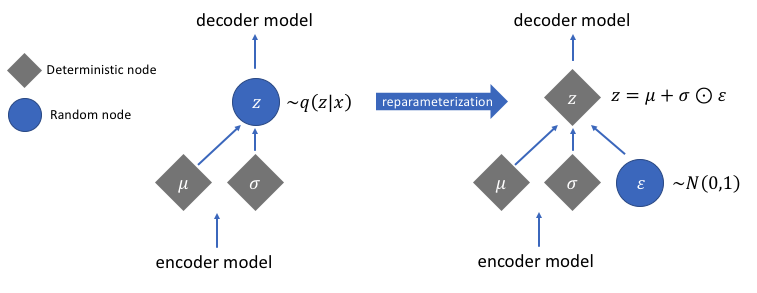
\includegraphics[width=\textwidth]{figures/background/reparametrization_trick.png}
    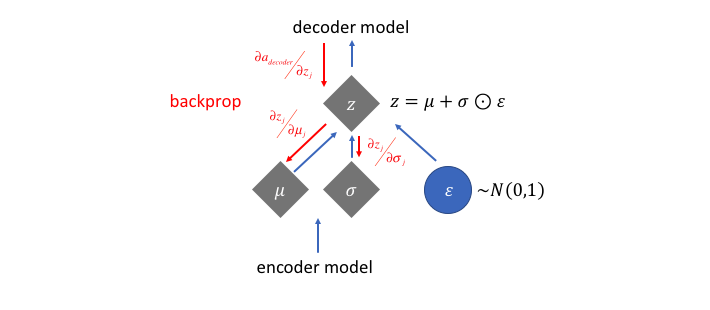
\includegraphics[width=\textwidth]{figures/background/reparametrization_trick_backprop.png}
    \caption{Comparing the data flow with and without reparametrization trick followed by the backprop calculation. Image source Note(\ref{note:jeremy_jordan})}
    \label{fig:reparametrization_trick}
\end{figure}

Hence the learned latent space of a \ac{vae} is continuous, while that of a standard autoencoder is discrete and clustered. As the decoder of the \ac{vae} is trained to generate data from this continuous space, it can generate realistic data by randomly sampling from this infinitely large latent space as illustrated in the Fig \ref{fig:vae_latent_attribute}. This also enables smooth interpolation of data produced from one point in the latent space to another. In addition to that, we can also perform arithmetics in vector space, similar to the popular example from Natural Language Processing, $King - Man + Women = Queen$ but on much higher dimensional embedding space.

\begin{figure}[h]
    \centering
    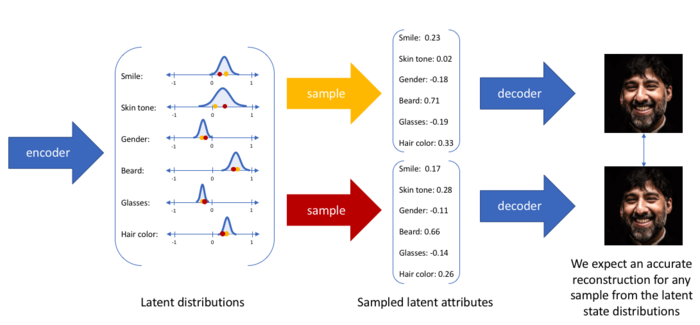
\includegraphics[width=\textwidth]{figures/background/vae_latent_attribute.png}
    \caption{Probabilistic distribution of latent attributes. Image source Note(\ref{note:jeremy_jordan})}
    \label{fig:vae_latent_attribute}
\end{figure}

\subsection{Beta Variational Autoencoder}
\label{subsec:bvae}
A \ac{vae} without the \ac{kld} term is effectively a standard autoencoder. As discussed the \ac{kld} term encourages the network to learn a distribution rather than a single value. If the variance of the distribution is not high, then it is again similar to an autoencoder. The more enforcement from \ac{kld}, the diverse the distribution. The \ac{vae} is forced to disentangle the representations, i.e the lesser is the correlation between each dimension in the latent space. Such disentangled representations are very useful for generative models. More importantly, it improves the interpretability of the latent space and can be leveraged to generalize to different downstream tasks. This emphasis on the latent space distributions can be achieved by disentangled variational autoencoders or \ac{bvae}, where $\beta$ is the weight coefficient of the \ac{kld} term in the \ac{vae} loss function Eqn.\ref{eqn:vae_loss}. So, the loss for the \ac{bvae} is $\mathcal{L}_{\mathrm{VAE}}$ Eqn. \ref{eqn:bvae_loss}. The higher the beta the stronger the constrain on the disentanglement. However, this constraint will negatively affect the representation capability of the \ac{vae}.

\begin{equation} \label{eqn:bvae_loss}
    \begin{gathered}[b]
        \mathcal{L}_{\mathrm{VAE}}=-\mathbb{E}_{q(z | x)} \log p(x | z) + \beta (D_{\mathrm{KL}}(q(z | x) || p(z)))
    \end{gathered}
\end{equation}

\subsection{Generative Adversarial Networks}
\label{subsec:gan}
\ac{gan} is an \ac{ann} that is used for generative tasks, to make the prediction \textit{realistic}. A \ac{gan} is a combination of 2 networks namely, the generator $G$ and the discriminator $D$. The generator learns to map a random sample or say, noise $Z$ drawn from a latent distribution with density $p_{z}$ to a higher dimensional data distribution with density $p_{g}$. Whereas the discriminator takes the output of the generator and tries to differentiate real data samples $x$ from the fakes which do not belong to the real distribution $p_{r}$  as illustrated in Fig \ref{fig:gan_arch}.

\begin{figure}[h]
    \centering
    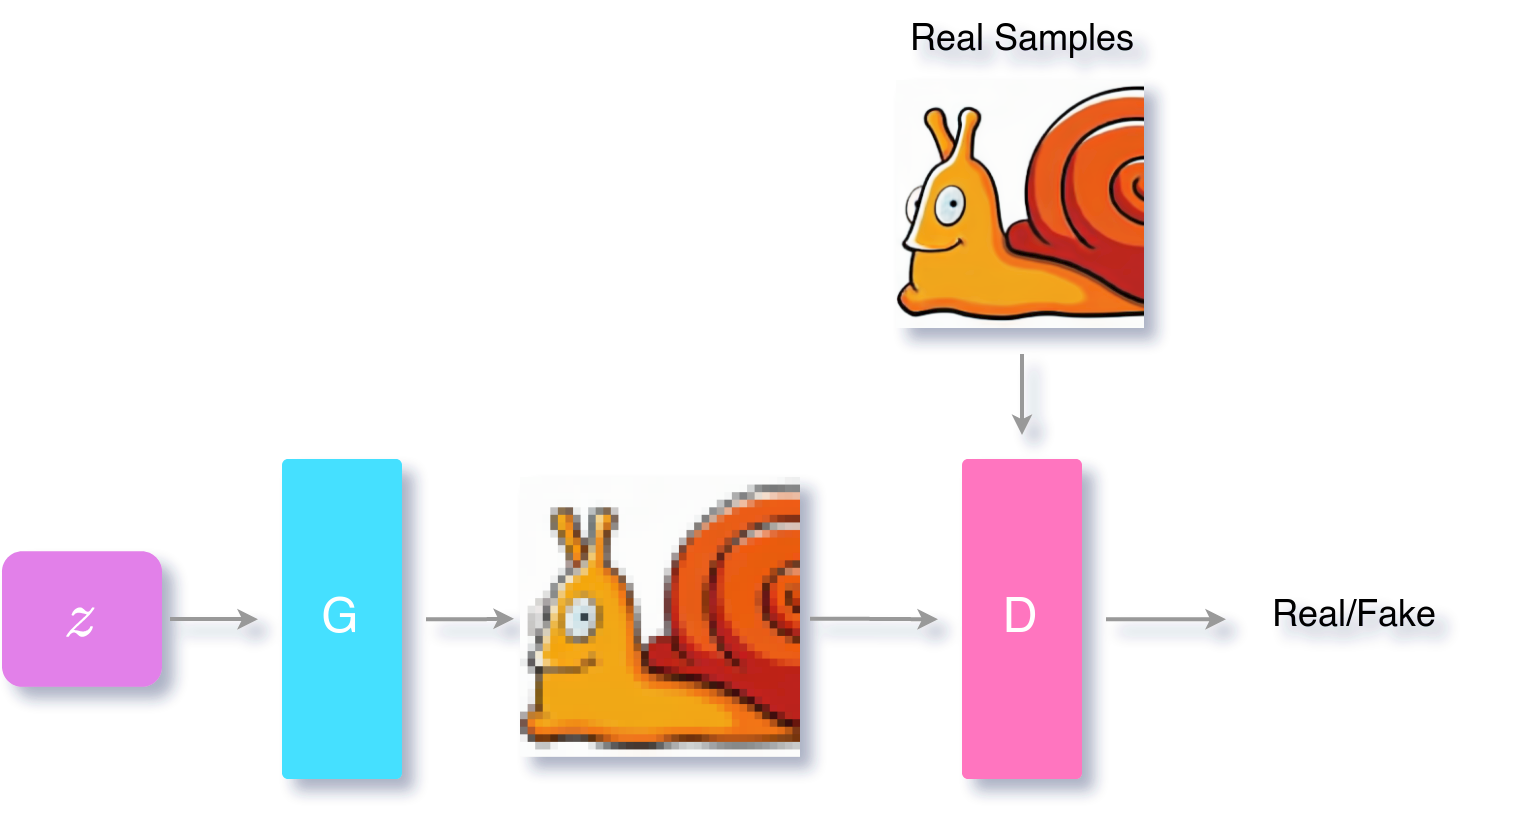
\includegraphics[width=0.7\textwidth]{figures/arch/gan_arch.png}
    \caption{Illustration of GAN architecture. G is the generator network and D is the discriminator network.}
    \label{fig:gan_arch}
\end{figure}

The goal of the generator is to produce samples, $G(z)$, that fool the discriminator into believing them as real samples. While the goal of the discriminator is to distinguish between the samples produced by the generator and the real samples by predicting reals as 1 and 0 for fakes. This inverse goal of the two networks can be viewed as a game of tug of war or a 2-player minimax game. The result of the game is that the generator would ideally learn to produce realistic data samples by sampling from prior $p_{g}(z)$. We effectively train $G$ to minimize $\log(1-D(G({z})))$ and $D$ to maximize $\log(D(x))$ making the loss function as $\mathcal{L}_{\mathrm{GAN}}$ Eqn. \ref{eqn:gan_loss}.

\begin{equation} \label{eqn:gan_loss}
    \begin{gathered}[b]
        {L}_{\mathrm{GAN}}=\mathbb{E}_{{x} \sim p_{r}(x)}[\log D({x})]+\mathbb{E}_{{z} \sim p_{z}(z)}[\log (1-D(G({z})))]
    \end{gathered}
\end{equation}

However, when it comes to training a \acp{gan}, practice is very different from theory. The training of the discriminator and generator is done iteratively and sequentially. But training the discriminator network to the optimal solution and then training the generator and repeating this loop is computationally challenging and would lead to overfitting the models on the finite dataset. To avoid this, the discriminator is trained for $k$ mini-batch iterations before training the generator for one iteration. This is to keep the discriminator close to optimality while slowly training the generator \cite{goodfellow2014generative}. The problem that arises here is that the generated samples are drastically different from the real samples as the generator has not yet learned to produce good samples. As the generator outputs samples close to noise, the discriminator easily distinguishes these samples from the real samples with high confidence. This saturates the loss term $\log (1-D(G(z)))$ very quick and leads to the problem of \textit{Vanishing Gradients}. Hence in practice, we train the generator $G$ to maximize $\log D(G(z))$ instead of minimizing $\log (1-D(G(z)))$, preventing the gradients from vanishing.

\begin{equation} \label{eqn:dg_of_x}
    \begin{aligned}[b]
        D_{G}^*(x) = & \frac{p_{r}(x)}{p_{r}(x)+p_{g}(x)} \\
        =            & \frac{1}{2}
    \end{aligned}
\end{equation}

At global optimality $p_{g}=p_{r}$, and for a given generator $G$, the discriminator at optimality is $D_{G}^*(x)$ Eqn. \ref{eqn:dg_of_x}. Hence the virtual cost $C(G)$ \cite{goodfellow2014generative} when $p_{g}=p_{r}$ is:

\begin{equation} \label{eqn:c_of_g}
    \begin{aligned}
        C(G) & = \max _{D} V(G, D)                                                                                                                                          \\
             & =\mathbb{E}_{x \sim p_{r}}\left[\log D_{G}^{*}(x)\right]+\mathbb{E}_{z \sim p_{z}}\left[\log \left(1-D_{G}^{*}(G(z))\right)\right]                           \\
             & =\mathbb{E}_{x \sim p_{r}}\left[\log D_{G}^{*}(x)\right]+\mathbb{E}_{x \sim p_{g}}\left[\log \left(1-D_{G}^{*}(x)\right)\right]                              \\
             & =\mathbb{E}_{x \sim p_{r}}\left[\log \frac{p_{r}(x)}{P_{r}(x)+p_{g}(x)}\right]+\mathbb{E}_{x \sim p_{g}}\left[\log \frac{p_{g}(x)}{p_{r}(x)+p_{g}(x)}\right] \\
             & =-\log (4)+ D_{\mathrm{KL}}\left(p_{r} \| \frac{p_{r}+p_{g}}{2}\right)+D_{\mathrm{KL}}\left(p_{g} \| \frac{p_{r}+p_{g}}{2}\right)                            \\
             & =-\log(4) + 2 \cdot  \mathrm{JSD}(p_{r} \| p_{g})
    \end{aligned}
\end{equation}

The \ac{jsd} \footnote{Jensen–Shannon divergence \url{https://en.wikipedia.org/wiki/Jensen-Shannon_divergence}} between two distributions is always non-negative and will be equal to zero only when both the distributions are equal. As we derived in Eqn. \ref{eqn:c_of_g} above, the best value of $C$ i.e $-\log 4$ is possible only when $p_{g}=p_{r}$. It is hard to stabilize the \ac{gan}'s minimax game \cite{martin2017principled}. It requires carefully tuned hyperparameters to maintain an equilibrium between the two players. Failing to find the proper balance between the networks leads to the problem of \textit{Non-Convergence}, where the training oscillates and never converge. When the generator is not strong enough and learns to produce samples that fool the discriminator, it eventually would restrict itself to only learn to produce such samples. This problem is referred to as \textit{Mode Collapse} \footnote{GAN Problems \url{https://developers.google.com/machine-learning/gan/problems}}. There are many hacks as well as principled approaches that are formulated to handle these problems with considerable success \cite{openaigan2wgan}.

\subsection{Wasserstein GAN}
\acp{wgan} is a variant of \acp{gan}, where the second network is a critic that scores the samples on how real they look rather than a discriminator that only predicts binary labels of 1 and 0 for real or fake. \ac{wgan} use 1-Wasserstein distance \footnote{Wasserstein Metric \url{https://en.wikipedia.org/wiki/Wasserstein_metric}} or \ac{emd} instead of the \ac{jsd} used in the standard discriminator based \ac{gan}. Since the Wasserstein distance is non-evaluative, a modified version Eqn. \ref{eqn:wasserstein_loss} of it is proposed as the loss function in \cite{soumith2017wasserstein}. Where $f$ being the critic network parameterized by $w$ while clipping the weights to satisfy the Lipschitz constraint.

\begin{equation} \label{eqn:wasserstein_loss}
    \begin{aligned}[b]
        L=\mathbb{E}_{x \sim P_{r}}\left[f_{w}(x)\right]-\mathbb{E}_{x \sim P_{g}}\left[f_{w}(x)\right]
    \end{aligned}
\end{equation}


% \begin{equation} \label{eqn:wasserstein}
%     \begin{aligned}[b]
%          W\left(P_{r}, P_{g}\right)=\inf _{\gamma \sim \Pi\left(P_{r}, P_{g}\right)} \mathbb{E}_{(x, x^\prime) \sim \gamma}[\|x-x^\prime\|]
% W\left(p_{r}, p_{g}\right)=\frac{1}{K} \sup _{\|f\|_{L} \leq K} \mathbb{E}_{x \sim p_{r}}[f(x)]-\mathbb{E}_{x \sim p_{g}}[f(x)]

%     \end{aligned}
% \end{equation}

%FIXME explain properly
% Where $\gamma \sim \Pi\left(P_{r}, P_{g}\right)$ is the collection of all possible joint distributions of $p_r$ and $p_g$. Adn for all the combinations the distance between the real sample$x$ and the generated sample $x^\prime$ can be calculated.   

The fundamental goal of \acp{gan} is to minimize the distribution between the real and the generated distribution. This could be measured used either of \ac{kld}, \ac{jsd}, \ac{emd}, or Wasserstein distance, the main difference being their impact on the convergence of these distributions. The interesting feature of the Wasserstein distance is that it is continuous and differentiable. Using this distance, the critic can train till optimality while having a reliable gradient throughout the training procedure. Hence the critic in \ac{wgan} does not have the saturation and vanishing gradient problems that exist in standard \acp{gan}. Due to continuous and clean gradients, the training is significantly stable and less sensitive to hyperparameters and model architecture. With \ac{wgan} the mode collapse problem is also significantly reduced. When it comes to practice, the most important problem that hinders training \acp{gan} is that there is no correlation between the quality of the generated data say, images, and the loss function. However, \ac{wgan} tries to converge the distributions while lowering the generation loss. And considerable relation between the loss and the quality of generations can be observed. \ac{wgangp} \cite{wgangp} is an improved \ac{wgan} that uses gradient penalty to enforce Lipschitz constraint.

\subsection{Hybrids - VAE-GAN}
\label{subsec:vaeganhybrid}
While the \acp{vae} learn the latent space of the data very efficiently, the generative capabilities are limited in comparison to \acp{gan}. In the case of image generations, \acp{vae} usually generate blurry images. While well trained \ac{gan} learn to generate photorealistic images. Though the task of the discriminator in \acp{gan} is to only learn what is real and what is fake, it implicitly learns rich a similarity metric in order do so \cite{autoencoding_beyond_pixels}. The idea of a \ac{vae}-\ac{gan}, illustrated in fig. \ref{fig:vae_gan_arch}, is to exploit this ability of \acp{gan} as a learning metric for \acp{vae} and the ability of \acp{vae} to learn dense latent representation of the data.

\begin{figure}[h]
    \centering
    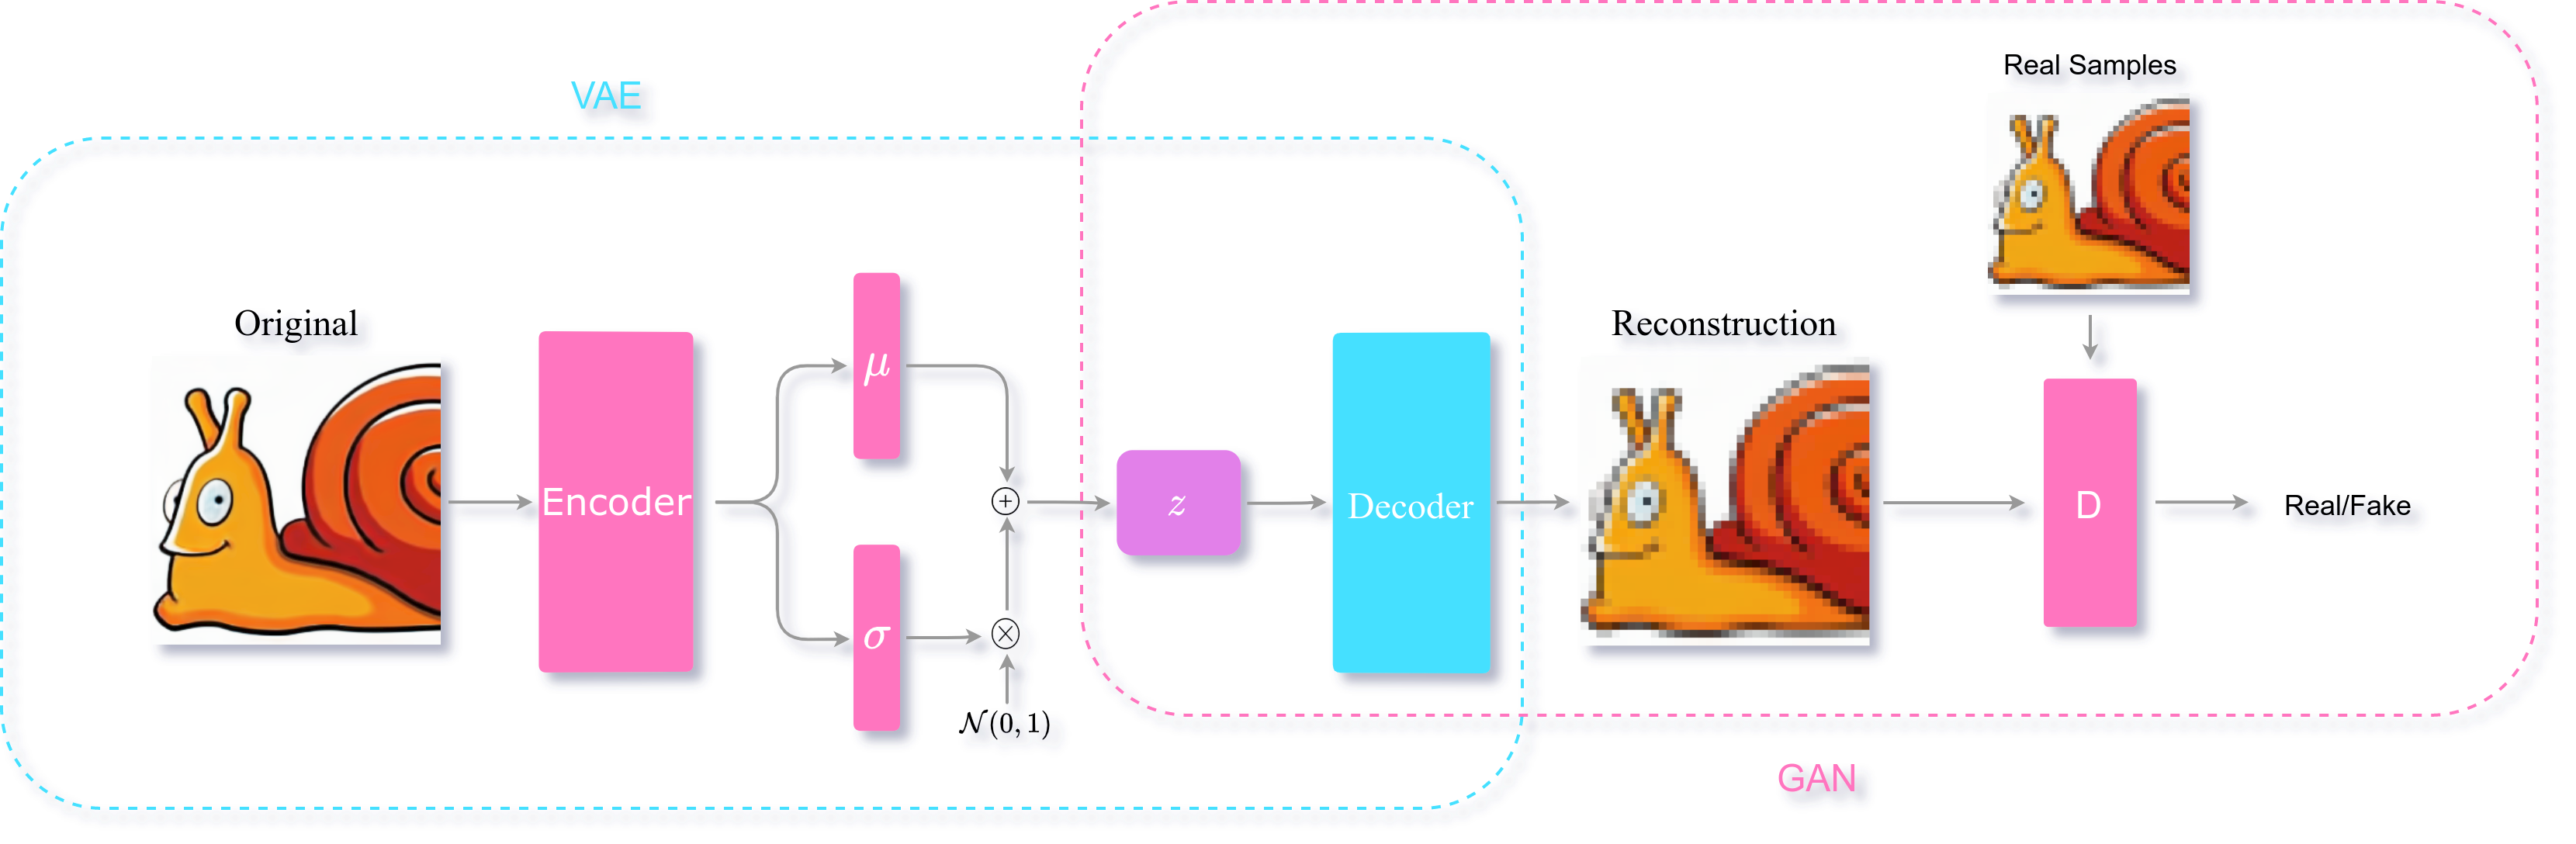
\includegraphics[width=\textwidth]{figures/arch/vae_gan_arch.png}
    \caption{Illustration of the \ac{vae}-\ac{gan} architecture}
    \label{fig:vae_gan_arch}
\end{figure}

Taking the example of images again, the element-wise error is a very poor similarity metric as a small deviation in a high-level feature, like eyebrow or head rotation would lead to high error as the pixel displacement propagates through huge parts of the image. These shifts, in reality, are plausible and realistic, probably indistinguishable from the human eye. Using the discriminator as a similar metric would address this problem as the error would be low for realistic deviations of features compared to unrealistic shifts say, the noise being upside down. This can be achieved by replacing the element-wise loss of the \ac{vae} Eqn. \ref{eqn:vae_loss} with the hidden representation $D_{l}(x)$ of an intermediate layer $l$ in the discriminator that would correspond to the hidden similarity metric. The Gaussian distribution for $D_{l}(x)$ is :
    
% TODO use operator name for D, G, and functions
\begin{equation} \label{eqn:gan_similarity}
    \begin{aligned}[b]
        p\left(D_{l}(x) | z\right)=\mathcal{N}\left(D_{l}(x) | D_{l}(\tilde{x}), I\right)
    \end{aligned}
\end{equation}

Where, $\tilde{x}$ is the generated sample from the \ac{vae}'s decoder $p$. $D_{l}(tilde{x})$ is the mean of the Gaussian distribution and $I$ is the identity covariance. Replacing this as the similarity metric in \ref{eqn:vae_loss}, we get the new $\mathcal{L}_{\text {recon}}$ :

\begin{equation} \label{eqn:vaegan_recon}
    \begin{gathered}[b]
        \mathcal{L}_{\text {recon}}^{D_{l}}=-\mathbb{E}_{q(z | x)} \log p\left(D_{l}(x) | z\right)
    \end{gathered}
\end{equation}

$\mathcal{L}_{\text {recon}}^{D_{l}}$ which uses the $l^{th}$ layer of the discriminator is only the metric for the \ac{vae}, the \ac{vae}-\ac{gan} is trained on a triplet loss \ref{eqn:vaegan_loss} with $\mathcal{L}_{\text GAN}$ from Eqn. \ref{eqn:gan_loss} as a \textit{style error}. Here the generator model is the same as the decoder of the \ac{vae} as it maps from $z$ to $x$ just like $G$.

\begin{equation} \label{eqn:vaegan_loss}
    \begin{gathered}[b]
    \mathcal{L}_{\mathrm{VAEGAN}} = \mathcal{L}_{\text {recon}}^{D_{l}} +\mathcal{L}_{\text {prior }} + \mathcal{L}_{\text {GAN}}
    \end{gathered}
\end{equation}

Training \ac{vae} is hard but training \ac{gan} is harder. It is very important to consider that the training of the \ac{vae} and the \ac{gan} takes place simultaneously. While doing so it is required to \textit{limit the error propagation} of the triplet loss to the entire model. The discriminator should not learn to minimize $\mathcal{L}_{\text {recon}}^{D_{l}}$, if it does, the discriminator collapses. Better results are observed by restricting the error signal to reach the encoder $q$ as illustrated in Fig. \ref{fig:vaegan_loss_graph}. 

\begin{figure}[h]
    \centering
    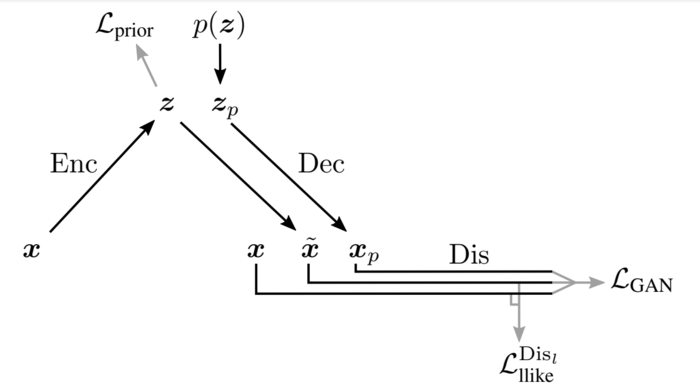
\includegraphics[width=0.8\textwidth]{figures/arch/vae_gan_loss_graph.png}
    \caption{Illustration of the data flow and the loss of \ac{vae}-\ac{gan}, where $\mathcal{L}_{\text {recon}}^{D_{l}}$ = $\mathcal{L}_{\text {llike}}^{Dis_{l}}$ \\
    Image source \cite{autoencoding_beyond_pixels}}. 
    \label{fig:vaegan_loss_graph}
\end{figure}

As discussed in \refsec{subsec:bvae}, \ac{vae} as a whole has two objectives - minimize the $\mathcal{L}_{\text {recon}}$ and the $\mathcal{L}_{\text {prior}}$ and a weighing factor $\beta$ is used to maintain a trade-off between the quality of the reconstruction and the extent of disentanglement. Similarly, when it comes to \ac{vae}-\ac{gan}, the decoder alone has two objectives. One is to generate samples minimizing the $\mathcal{L}_{\text {recon}}^{D_{l}}$ and the other is to make sure that the generated samples can fool the discriminator. And the trade off is regulated by using $\gamma$ to weigh $\mathcal{L}_{\text {recon}}^{D_{l}}$ and $\mathcal{L}_{\text {\ac{gan}}}$ as in Eqn. \ref{eqn:vaegan_gamma}.
 
\begin{equation} \label{eqn:vaegan_gamma}
    \begin{gathered}[b]
        \theta_{p} \stackrel{+}{t}-\nabla_{\theta_{p}}\left(\gamma L_{\mathrm{uike}}^{D}-\mathcal{L}_{\mathrm{GAN}}\right)
    \end{gathered}
\end{equation}

In the standard \ac{gan} training, samples from the prior $p(z)$ are passed to the decoder which generates samples that are then passed to the discriminator. Interesting observation when using \ac{vae}-\ac{gan} is, sampling $x$ from the encoder $q(z|x)$ further improves the results. As the \ac{vae} tries to minimize $\mathcal{L}_{\text{prior}}$, the samples from $p(z)$ and $q(z|x)$ become similar during the training. As the generated samples $p(q(z|x))$ using the encoder are more realistic than $p(p_{prior}(z))$ using the prior, they serve as better adversarial examples for the discriminator. The $\mathcal{L}_{\mathrm{GAN}}$ loss to be used to leverage this benefit is: 

%FIXME change decoder p to be different from prior 

\begin{equation} \label{eqn:vaegan_ganloss}
    \begin{gathered}[b]
        \mathcal{L}_{\mathrm{GAN}}=\log (Dis(x))+\log (1-Dis(Dec(z)))+\log (1-Dis(Dec(Enc(x))))
    \end{gathered}
\end{equation}

%FIXME WGAN is wrong

%%%%%%%%%%%%%%%%%%%%%%%%%%%%%%%%%%%%%%%%%%%%%%%%%%%%%%%%%%%%%%%%%%%%%%%%%%%%%%      RELATED WORKS      %%%%%%%%%%%%%%%%%%%%%%%%%%%%%%%%%%%%%%%%%%%%%%%%%%%%%%%%%%%%%%%%%%%%%%%%%%%%%%%%%%%%%%%%%%%%%%%
\section{Research Area Introduction}
\label{sec:Research area introduction}

In this section, the details of various approaches and the \ac{sota} in 3D \ac{hpe} are presented along with some works in the sibling tasks of hand pose estimation. This section aims to only give an overview of how the problem of 3D \ac{hpe} is tackled in the literature, approaches that are directly related to the method proposed in this thesis are presented later in section \refsec{sec:Related Work}, Related Works. The different categories of the approaches mentioned below are not exclusive but are the main aspects of the described approaches.

\subsection{Cascading Approach}

Numerous works try to estimate 3D human poses from 2D RGB images or 2D joint confidence heatmaps \cite{CameraDistanceAware, poselifter, DistillNRSfM, occlusionVideo, ordinalranking}. Most of these methods follow a cascading approach, where an explicit intermediate representation of 2D heatmaps or 2D poses is predicted. This typically involves training a convolutional neural network to find humans in the image or just extract features that correspond to the joints. These features are forwarded to another neural network that learns to estimate the corresponding 3D pose, usually by predicting the depth offsets of the 2D joint or sometimes by predicting the shape and the view parameters of the 3D pose.

For example, \cite{CameraDistanceAware} proposes a general framework with 3 networks as depicted in Fig \ref{fig:CameraDistanceAware}. Human detection Network, RootNet, PoseNet. Where the human detection network predicts the region the human is in an image. The RootNet localizes the human's root in the global 3D world. And, the PoseNet predicts the 3D pose of a single person relative to the root. Where the root is a fixed reference point of the human body says, the pelvis.

\begin{figure}[h]
    \centering
    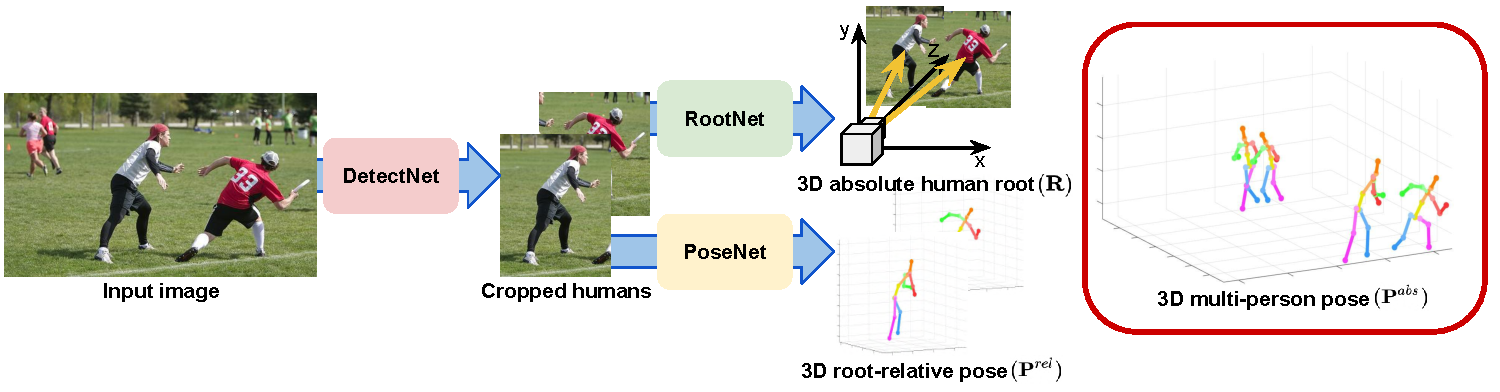
\includegraphics[width=\linewidth]{figures/background/cascading_arch.pdf}
    \caption{Pipeline of an absolute 3D \ac{hpe} network following a cascading approach \cite{CameraDistanceAware}, showing different neural networks such as DetectNet, RootNet and PoseNet that trained on specific subtasks to estimate absolute 3D human pose.}
    \label{fig:CameraDistanceAware}
\end{figure}

The advantage of such top-down frameworks is the possibility to divide the task of RGB to 3D into smaller, well-studied sub-tasks. This enables explicit supervision of know intermediate states that could be of interest for understanding the representations learned by the network or to use the intermediate output for other auxiliary tasks. Moreover, in this case, it makes scaling single-person pose estimation algorithms for multi-person pose estimation easy, as the majority of the data available mostly consists of a single person per frame. Most importantly certain modules can be replaced or improvised without affecting or having to re-train the entire pipeline.

\subsection{Pose Lifting}

In contrast to the estimating pose from an image, Pose Lifting works such as \cite{poselifter,  amazon1, repnet, c3dpo, unsupervisedAdversarial}, focus on estimating 3D poses from 2D poses alone while assuming 2D poses from the \ac{sota} methods in 2D \ac{hpe}. This category follows the idealogy of cascading based approaches but restricts the study and discussion purely to lifting 2D to 3D pose. These methods include simple linear models as first described in \cite{MartinezHRL17} with a series of fully connected linear, batch normalization, dropout layers with residual connections as illustrated in Fig \ref{fig:lifting_arch} to regress 3D pose effectively. These simple networks have enough capacity to capture the features of the data as the input and output data are much smaller in dimensions as compared to RGB images.

\begin{figure}[h]
    \centering
    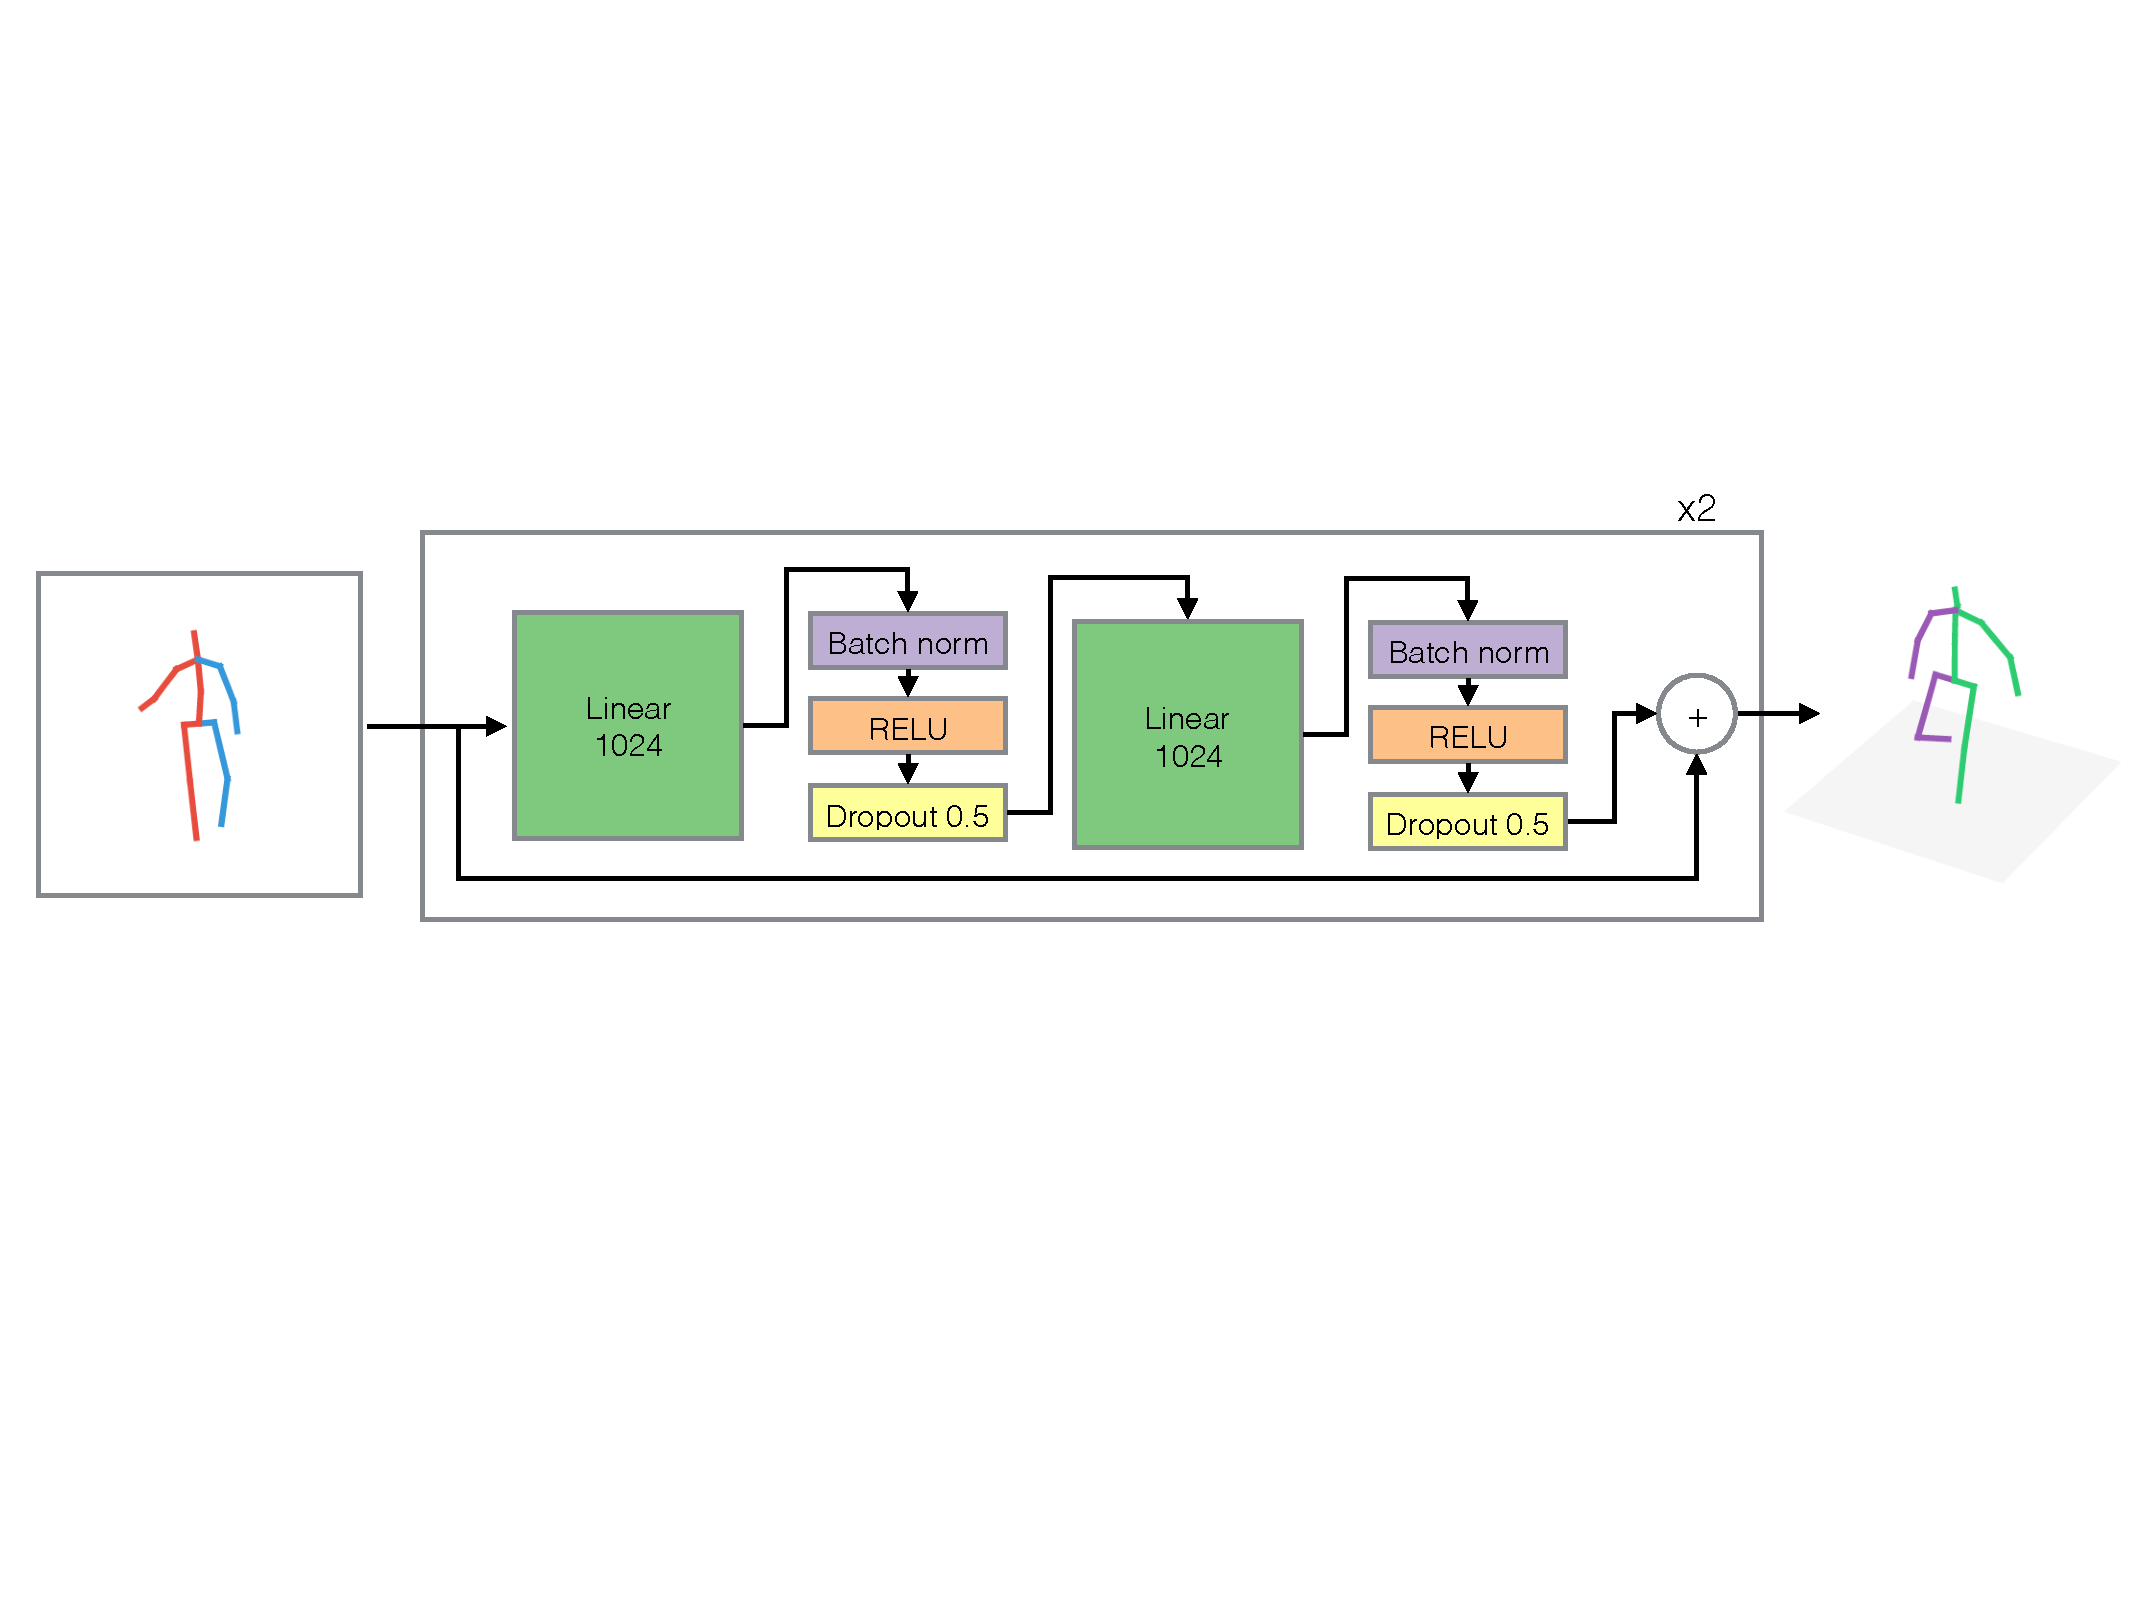
\includegraphics[width=\linewidth]{figures/background/lifting_arch.pdf}
    \caption{Architecture of the first deep learning based lifting appraoch proposed by Martinez \etal \cite{MartinezHRL17}}
    \label{fig:lifting_arch}
\end{figure}

\ac{nrsfm} is another promising lifting method that also leverages images along with 2D annotations. \ac{nrsfm} deals with the problem of reconstructing 3D shape (pose/point cloud) and cameras of each projection from a sequence of images with corresponding 2D projections (2D keypoints). This approach has been widely used in facial keypoint detection and \cite{deepNRSFM} introduces a deep learning variant for the same. Instead of predicting the 3D coordinates of each keypoint/joint of the 3D pose, \cite{DistillNRSfM, c3dpo, deepNRSFM, nrsfm++} predicts the 3D shape and camera pose from 2D pose using this method. The advantage of such an approach is to obtain a disentangled representation of view and 3D pose that is invariant of the view or camera position.

The Lifting approaches facilitate to leverage of the already well established 2D \ac{hpe} models that are trained on enormous and diverse labeled data. Thus demanding lesser training data for 3D pose estimation than it would need when learning from images. Since these networks do not have large convolution layers they are computationally inexpensive for both training and inference. Moreover, the 2D and 3D pose data usually can be entirely loaded onto the GPU further accelerating the training procedure. Thus addressing one of the major problems that affect the scalability of 3D \ac{hpe} models as well as enabling the development of better modular systems by combining the best of Lifting networks with the best of 2D \ac{hpe}.

\subsection{Multiple Hypothesis Estimation}
\label{subsec:multiple_hypothesis_estimation}

As stated in \refsec{sec:background}, 2D-to-3D pose lifting is an ill-posed-inversed problem due to inherent depth ambiguity as multiple plausible 3D poses give the same 2D projection, this shall be further elaborated later in Chapter \ref{chap:data}, Data. To address this problem, Jahangiri \etal \cite{jahangiri} propose a solution a 3D \ac{gmm} to learn uniformly sampled 3D poses and conditionally sample to retrieve 3D poses that have the reprojection error within the given limits. Thus estimating multiple 3D poses conditioning on a single input 2D pose, similar to a dictionary-based learning approach. 

More deep learning-based approaches such as \cite{weaklymultiple,multiplehypo,ordinalranking} were later introduced. Out of them, Chen Li \etal \cite{multiplehypo} proposes a variational inference model replacing the \ac{gmm} with a \ac{mdn} which was first introduced by Ye \etal \cite{mixturedensitymodel} to handle occlusions in hand pose estimation. Thus addressing two of the major problems of 3D \ac{hpe} i.e missing joints from occlusions and variational inference. 

Another interesting approach from Sharma \etal \cite{ordinalranking}, presents a conditional \acl{vae} which takes a random sample from a normal distinguish as input and 2D pose as a condition and outputs different 3D pose for different random samples given the same 2D pose. This approach also handles missing joints and provides variational inference. An evaluation technique is also proposed to rank each of the multiple hypotheses by scoring the poses based on joint-ordinal depth relations learned from the images or by oracle score that access 3D ground truth to compute the closest match as illustrated in Fig \ref{fig:ordinal_arch}.

\begin{figure}[h]
    \centering
    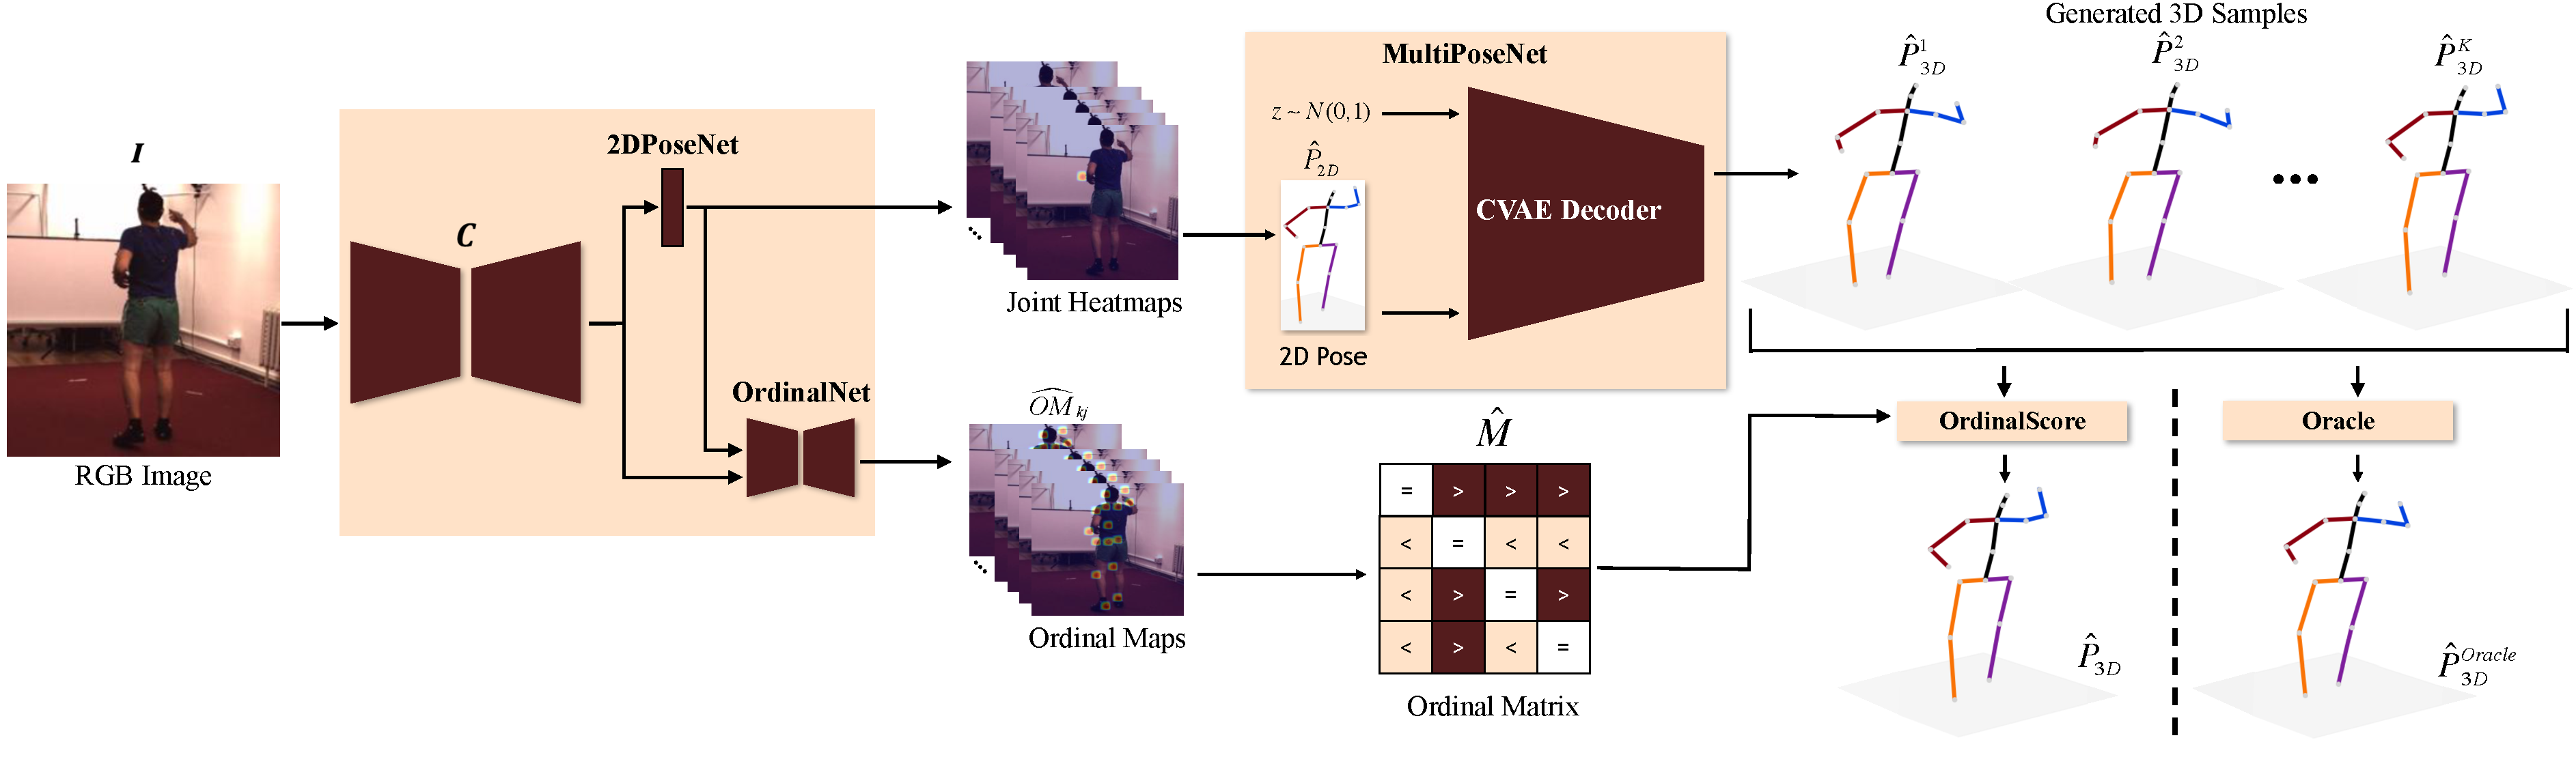
\includegraphics[width=\linewidth]{figures/background/ordinal_arch.pdf}
    \caption{Illustration of modular framework from \cite{ordinalranking} that uses a Conditional \ac{vae} to estiamte multiple hypothesis for a given 2D pose as condition. The ordinal scoring learnt from joint-depth ordinal relations and the score obtained from the oracle that learns scores higher to poses closest to the ground truth pose are used rank to each of the predicted 3D pose.}
    \label{fig:ordinal_arch}
\end{figure}

Recent work from Chen Li \etal \cite{weaklymultiple} which is an improvised version of their earlier work \cite{multiplehypo} proposes a weakly supervised approach that is much more similar to that of this thesis. The details are discussed later in the related works section \refsec{sec:Related Work}. However, all of the mentioned approaches still require 3D poses in one way or other for training and hence do not address the most important bottleneck of obtaining 3D ground truth. 

\subsection{Non-Supervised Learning}
\label{subsec:non_supervised_learning}
The standard way to train 3D/2D \ac{hpe} is by minimizing the distance between the predicted 3D/2D pose and its corresponding 3D ground truth. The area of 2D \ac{hpe} is well established and matured with reliable systems deployed in the real world. This was made possible with the high volume of images from diverse settings and the reasonable ease of manual labeling of 2D poses. On the other hand, labeling 3D pose manually is not practical. Though single-person datasets such as Human3.6M \cite{H3.6}, Human Eva \cite{HumanEva} and, multi-person datasets such as CMU Panoptic \cite{cmuPanoptic} provide 3D pose ground truth, they are obtained using \ac{mocap} systems Fig[\ref{fig:h36_mocap}] which are only limited to indoors or cannot be directly adapted to outdoor environments where the majority of the use cases exist. It is also worth mentioning JTA (Joint Track Auto) dataset \cite{JTA} that is made using the GTA(Grand Theft Auto) game engine which is technically scalable with its limitations. The datasets from simulations come with the difficulty of domain adaptation to be transferable to the real world.

\begin{figure}[h]
    \centering
    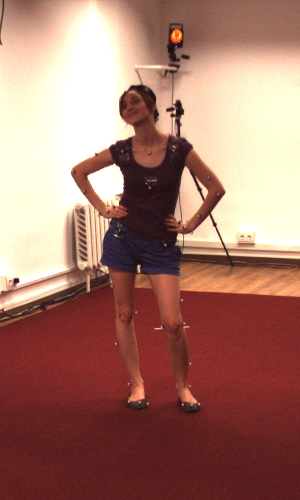
\includegraphics[width=30mm]{figures/h36/h36_mocap.png}
    \caption{Image from Human3.6 Dataset \cite{H3.6} of subject wearing \ac{mocap} markers}
    \label{fig:h36_mocap}
\end{figure}

To overcome this bottleneck, \cite{unsupervisedAdversarial} proposes unsupervised training of a generative adversarial network by projecting the predicted 3D pose back to 2D and minimizing its distance with the input 2D pose. And further training a discriminator to distinguish the real 2D pose from the projected poses as illustrated in Fig \ref{fig:adverserial_arch}. Thus removing the need for any explicit 3D annotations besides 2D pose that are either manually labeled or obtained using 2D \ac{hpe} models. RepNet \cite{repnet} trains an adversarial network without 2D-3D correspondences in a weakly supervised manner. Moreover, it also does not require camera parameters to project the 3D pose but learns to predict them. Thus enabling better generalization to more diverse data with unknown cameras and poses.

\begin{figure}[h]
    \centering
    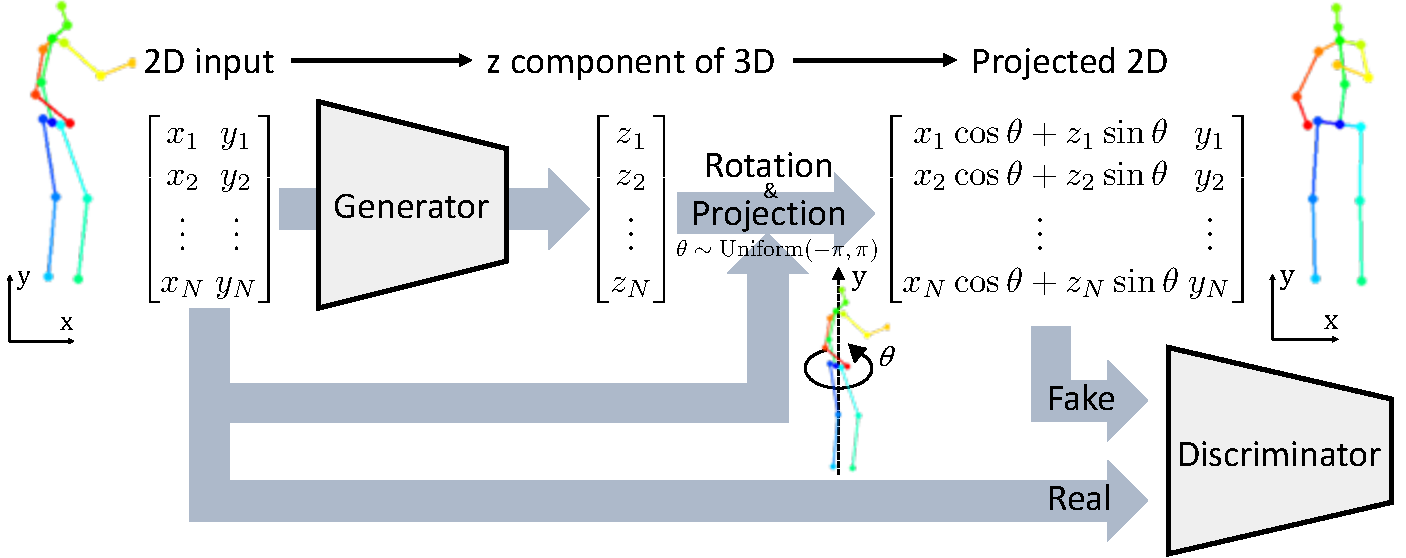
\includegraphics[width=\linewidth]{figures/background/adverserial_arch.pdf}
    \caption{Architecture of a simple unsupervised adversarial learning architecture proposed by \cite{unsupervisedAdversarial}. The network takes 2D coordinates ($x$, $y$) of each joint in the pose and predicts the corresponding $z$-component. The 3D pose achieved by combining the input $x$, $y$ with the predicted $z$, is randomly rotated along the $y$-axis to retrieve a novel view of the 3D pose. This pose is the projected to $xy$-plane, which would be much different from the input 2D pose. This projected 2D pose should be similar to the real 2D poses in the dataset if the predicted 3D represents the true human pose. Their similarity to real 2D poses is reinforced by a discriminator. The whole training produce is carried out without the need for a 3D pose in any shape or form.}
    \label{fig:adverserial_arch}
\end{figure}

To test the maximum capability of Pose Lifting networks, \cite{amazon1} proposes a combination of unsupervised and adversarial learning that mainly leverages the property of \textit{plane-invariance}. It is the property that 2D projections of a 3D pose from different camera viewpoints, when lifted should produce identical and the original 3D pose. In this method, the predicted 3D pose is rotated in random angles and is reprojected to 2D in a different \ac{pov}. A discriminator is then used to evaluate if this new 2D pose is in the possible pose distribution which is learned from 2D pose datasets alone. These steps are redone in reverse order to obtain the original 2D input. This cycle provides three intermediate representations of the single 2D input that the models learn from. Additionally, this approach exploits the temporal consistency in the datasets as well as integrates a domain adaptation network to learn from different datasets and distributions to achieve comparable results to that of the methods that require more supervision. However, due to the inherent ambiguity in lifting 2D pose to 3D and as the images are not captured with orthogonal cameras, reprojection of 3D pose is not necessarily consistent with the ground truth as the camera intrinsic and extrinsic parameters are not taken into account. Hence it is challenging to match the performance of models trained on 3D ground truth.

\subsection{Multimodal Representation Learning}
\label{subsec:multimodal_representation_learning}

Another interesting approach is training \ac{vae}s using multiple modalities like images, poses, depth maps \cite{CrossingNets, crossmodal, MMVAE, HandDisentangled}. \ac{mvae}s learn representation from different modalities in the same latent space. True multimodal learning needs to fulfill 4 criteria as follows: i) \textit{Latent Factorization} - Implicit factorization of latent space into private, shared subspaces based on modality as illustrated in the figure[\ref{fig:criteria}]. ii) \textit{Coherent Joint Generation} - Coherence in generations of different modalities from the same latent value with respect to the shared aspects of the latent. iii) \textit{Coherent Cross Generation} - Generation of one modality conditioned on data from different modality while preserving the similarity between them. iv) \textit{Synergy} - Enhancement in generation quality of one modality as a result of learning representations of different modalities.

\begin{figure}[h]
    \centering
    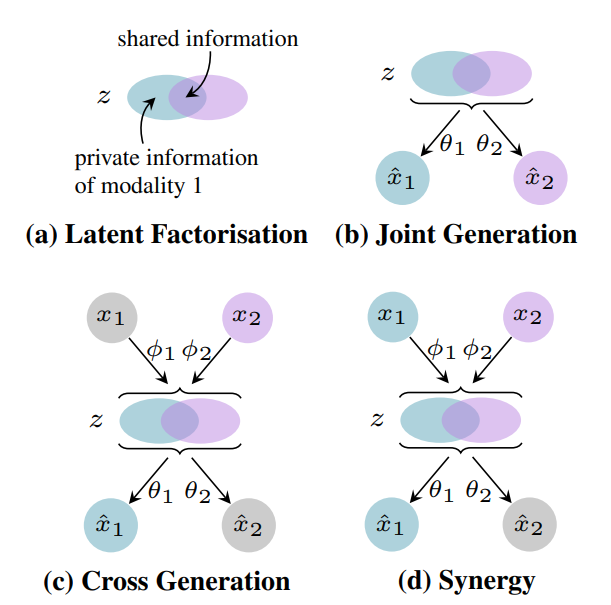
\includegraphics[scale=0.5]{figures/background/criteria.png}
    \caption{Criteria for Multimodal Generation \cite{MMVAE}}
    \label{fig:criteria}
\end{figure}

\ac{mmvae} proposed by \cite{MMVAE} fulfills all 4 of the above-mentioned criteria learning representations of image and text data, while other approaches focus on leveraging specific advantages of multimodal learning. Consider the cross-modal learning for 3D Hand Pose Estimation proposed by \cite{crossmodal}. It involves training an encoder-decoder pair to learn image representation, and another such pair to learn 3D hand pose representations in the same latent space. This training procedure focuses on cross-generation and synergy. That is, using the shared latent space of the image and pose representations, the RGB image encoder combined with the pose decoder can generate 3D poses and vice versa while preserving the commonality between the conditioned and the generated data. With this approach, it is possible to train a \ac{vae} for 3D \ac{hpe} from RGB images without explicit intermediate stages like the earlier mentioned cascading approaches. Making it more efficient and fast for both training and inference without compromising the modularity offered by cascading approaches.

\section{Related Work}
\label{sec:Related Work}

In this section, works that are directly related to the thesis are discussed in more detail. Some are the best examples of their kind and have already been discussed thoroughly. The basic idea of the thesis is to learn 3D \ac{hpe} just from 2D pose data without using 3D ground truth in any shape or form. Thus developing a method that can exploit the huge amounts of 2D pose data that can be generated using state of the art 2D pose networks on diverse images from the real world. The following approaches use weakly supervised or unsupervised approaches to accomplish the same. These serve as the inspiration for many of the choices taken in this thesis and also help understand the possibilities of reducing the need for explicit 3D supervision.

To the best of knowledge acquired during the period of the thesis, \cite{can3dpose, amazon1, unsupervisedAdversarial, c3dpo} are the main approaches that do not use 3D supervision in any way. While \cite{repnet, weaklymultiple} are among the main approaches that use 3D supervision to train the discriminator alone. The approaches that are not mentioned are either the approaches the above mentioned are built up or have been missed during the literature study or most likely published after finishing this thesis report.

\cite{unsupervisedAdversarial, can3dpose, amazon1} can be viewed as a series of approaches that are built on one another in the same order. They take 2D poses as the input and learn to predict the depth offset for each joint to reconstruct 3D. Out of the three Ching \etal \cite{amazon1}, using the plane invariance, geometric self-supervision, and adversarial learning as discussed earlier in \refsec{subsec:non_supervised_learning}, achieves the \ac{sota} results compared to fully supervised methods and also present ways to use domain adaptation network, temporal consistency to further integrate more datasets and improve the performance. Thus directly address the hurdles of scaling the 3D \ac{hpe} network to the real world. However, they also acknowledge the fact that most of the predictions made by \ac{sota} 2D \ac{hpe} model on real-world images have missing joints. Since the proposed approaches only predict the depth of every joint, the error from the 2D input pose is directly propagated to the 3D prediction. More importantly, it is not possible to use most of the data that is generated from 2D pose models. Hence it is very crucial to handle the problem of \textit{\textbf{missing joints}} to truly unlock the potential of unsupervised learning.

Wandt \etal \cite{repnet} also mentioned in \refsec{sec:Research area introduction} proposes an architecture that learns to predict the whole 3D pose, while also learning the camera parameters that are used to project the predicted 3D to 2D. The idea behind the camera parameter network is to learn the view angle given pose to generalize to unknown cameras. The pose network learns to converge the predicted 2D reprojections while using a \ac{gan} trained on \textit{\textbf{3D ground truth labels}} to supervise the predicted 3D pose. Though there is no direct error propagation from 2D input to 3D, it is important to note the problem of missing joints is not yet addressed. However, there another fundamental problem of \textit{\textbf{depth ambiguity}} persists. 

\begin{figure}[h] 
    \centering
    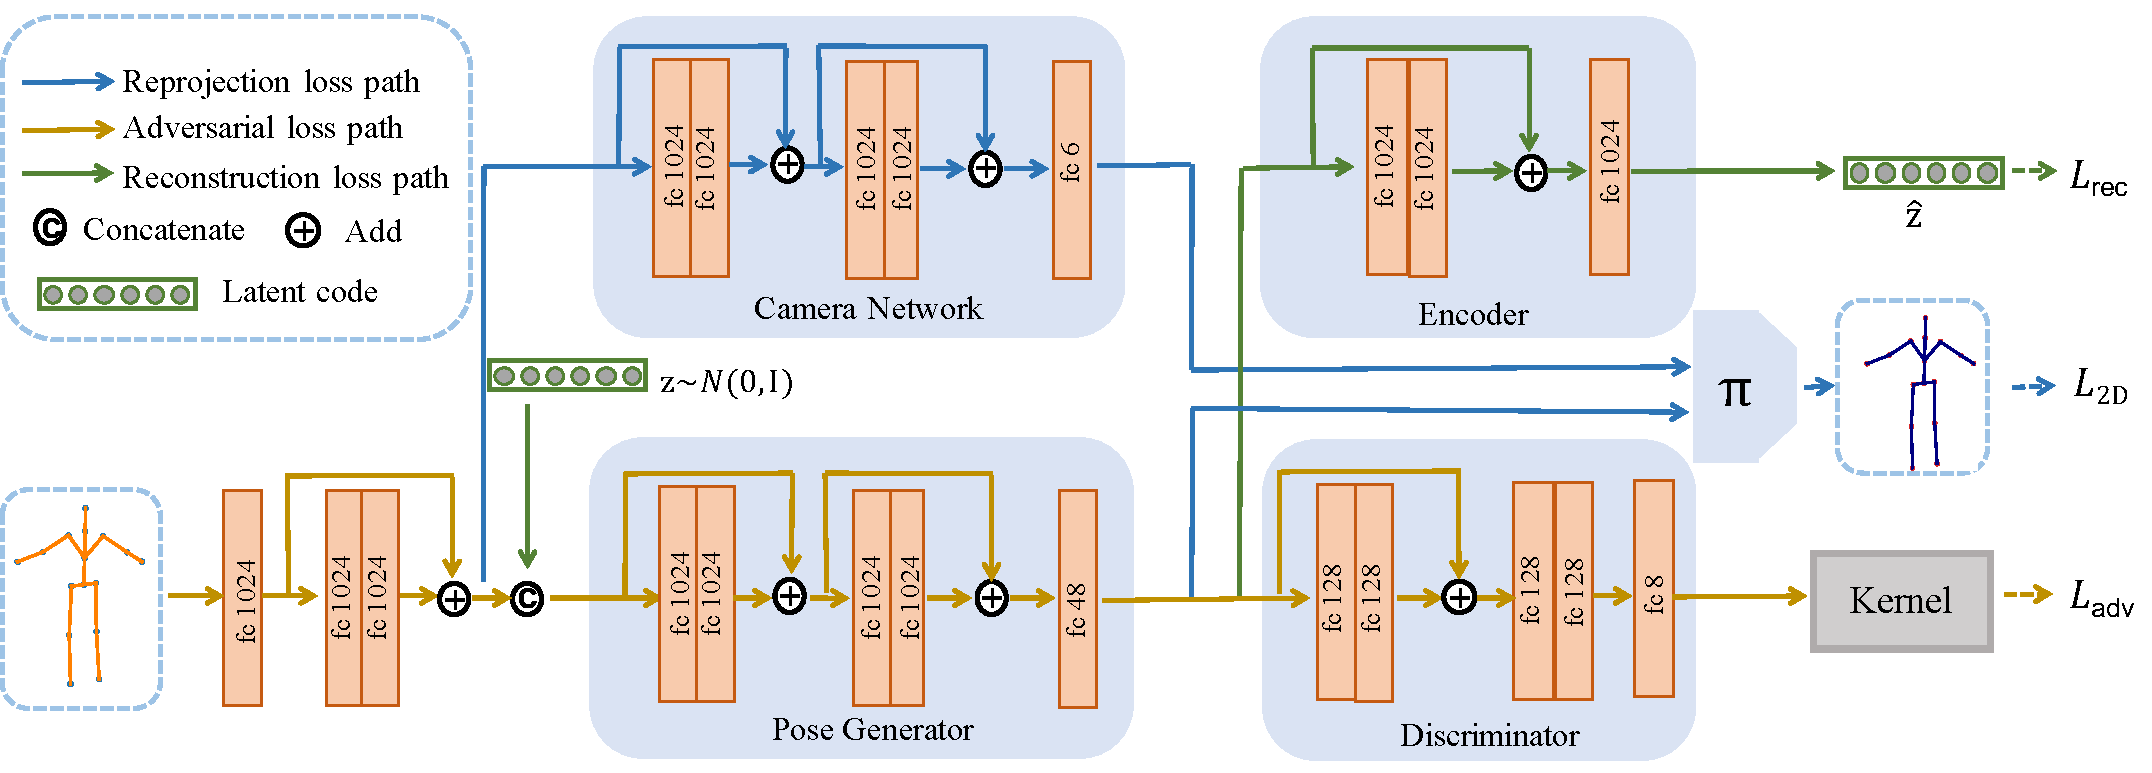
\includegraphics[width=\linewidth]{figures/background/multi_arch.pdf}
    \caption{Illustraion of the weakly supervised multiple hypothesis generation architecture proposed by \cite{weaklymultiple}}
    \label{fig:multi_arch}
\end{figure}


Chen Li \etal \cite{weaklymultiple}, building upon their previous work \cite{multiplehypo} that is explained earlier in \refsec{subsec:multiple_hypothesis_estimation}, proposes a weakly supervised variational inference model as the proposed method in this thesis was developed. The new approach \cite{weaklymultiple} was inspired by the architecture of Wandt \etal \cite{repnet} that does not require direct 3D supervision. This model first encodes the input 2D pose to a latent representation. This representation is then concatenated with a \textit{latent code} to produce a 3D pose as well as used by the camera network to predict the camera pose. Instead of directly supervising the predicted 3D pose with the ground truth, it is projected back to 2D using the predicted camera view which is self-supervised as it should be the same as the input 2D pose. 

This self-supervision trains the network to only output 3D poses that are close to input 2D in a particular view but unconstrained from another view. To ensure, the predicted 3D is feasible and close to ground truth a \ac{wgan} is used as illustrated in Fig \ref{fig:multi_arch}. The predicted 3D pose is passed to a critic network that scores the poses on how realistic they are. This encourages the pose network to generate poses that are realistic, in other words, indistinguishable from the 3D ground-truth poses. This results in a realistic 3D pose that is close to the 2D input pose which is most likely close to its corresponding 3D ground truth. In addition to this, an encoder is trained to reconstruct the latent code to ensure diversity and prevent mode collapse of the \ac{wgan}. 

This variational inference of 3D pose addresses both the problems of depth ambiguity and missing joints. However, this weakly supervised still requires 3D ground truth poses to train the discriminator and does not address the problem completely. The method proposed in this thesis is similar to this approach but does not require 3D in any shape or form, and uses much smaller architecture without the camera and latent vector encoder networks while addressing all the major problems. 

Canonical 3D Pose Networks for Non-Rigid Structure From Motion (C3DPO) \cite{c3dpo}, which is also discussed in \refsec{subsec:non_supervised_learning} handles missing joint and is fully unsupervised but does not have the capability of predicting multiple hypotheses for a given 2D pose. This approach that uses \ac{nrsfm} in an unsupervised way, does not yield good results compared to other approaches. In this thesis, we present a method that has the merits of the above approaches and addresses all the aforementioned problems.